\documentclass{report}
\usepackage{tikz}
\usepackage{amsfonts}

\usetikzlibrary{decorations.pathreplacing}
\usepackage{subcaption}

\begin{document}
\begin{figure}
  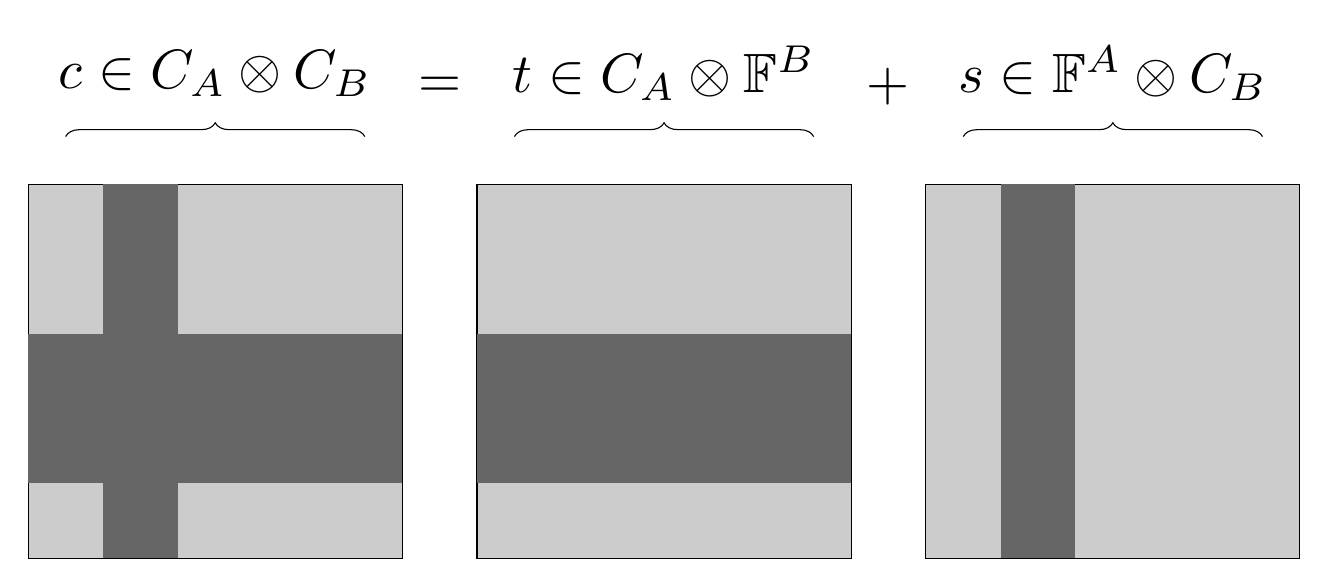
\begin{tikzpicture}[scale=0.95]

    \draw (5.5,6.3) node[scale=2]  { $=$ };
    \draw (11.5,6.3) node[scale=2]  { $+$ };

\draw [decorate,decoration={brace,amplitude=5pt,raise=4ex}] 
(0.5,5) -- (4.5,5) node[scale=2,midway,yshift=2em]{$c \in C_{A}\otimes C_{B}$};
        \filldraw [fill=white!80!black](0,0) rectangle (5,5);
       \fill [fill=gray!80!black] (1,0) rectangle (2,5);
        \fill [fill=gray!80!black] (0,1) rectangle (5,3);
\filldraw [fill=white!80!black](6,0) rectangle (11,5);
 \draw [decorate,decoration={brace,amplitude=5pt,raise=4ex}] 
 (6.5,5) -- (10.5,5) node[scale=2,midway,yshift=2em]{$t \in C_{A}\otimes \mathbb{F}^{B}$};
       \fill [fill=gray!80!black,draw opacity=0.5] (6,1) rectangle (11,3);
\filldraw [fill=white!80!black](12,0) rectangle (17,5);
  \draw [decorate,decoration={brace,amplitude=5pt,raise=4ex}] 
  (12.5,5) -- (16.5,5) node[scale=2,midway,yshift=2em]{$s \in \mathbb{F}^{A}\otimes C_{B}$};
     \fill [fill=gray!80!black,draw opacity=0.5] (13,0) rectangle (14,5);
            \end{tikzpicture}
\end{figure}
\end{document}
